\chapter{Elementary Conformal Mappings}
\label{chap:elementary-conformal-mappings}

The conformal mapping associated with an analytic function affords an excellent visualization of the function's behavior; it can be well compared with the visualization of a real function by its graph. It is therefore natural that all questions connected with conformal mapping have received a great deal of attention. In addition, conformal mapping enters naturally in many branches of mathematical physics ad in this way accounts for the immediate usefulness of complex-function theory.

\section{The Use of Level Curves}
When a conformal mapping is defined by an explicit analytic function $w=f(z)$, we naturally wish to gain information about the specific geometric properties of the mapping. One of the most fruitful ways is to study the correspondence of curves induced by the point transformation. The special properties of the function $f(z)$ may express themselves in the fact that certain simple curves are transformed into curves of a family of well-known character. Any such information will strengthen our visual conception of the mapping.

For example, in the case of linear transformations -- which are the easiest to understand -- we proved that they carry circles to circles, provided that we extend the definition of circle to include straight lines, as well. By consideration of the Steiner circles it was possible to obtain a complete picture of the correspondence.

In more general cases it is advisable to begin with a study of the image curves of the lines $x=x_0$ and $y=y_0$, where $x_0$ and $y_0$ are constants. If we write $f(z)=u(x,y)+iv(x,y)$, then the image of the line $x=x_0$ is given by the parametric equations $u=u(x_0,y)$ and $v=v(x_0,y)$, where $y$ varies. Similarly, the image of the line $y=y_0$ is given by $u=u(x,y_0)$ and $v=v(x,y_0)$. Together the curves form an orthogonal net in the $w$-plane. Similarly, we may consider the curves $u(x,y)=u_0$ and $v(x,y)=v_0$ in the $z$-plane; they are also orthogonal and are called the \emph{level curves} of $u$ and $v$. Moreover, the modulus and argument of an analytic function are orthogonal by way of the geometric fact that the radius of a circle is perpendicular to a tangent at the point of tangency..

In other cases it may be more convenient to use polar coordinates and study the images of concentric circles and straight lines about the origin.

Among the simplest mappings are those by a power $w=z^{\alpha}$, where $\alpha$ is real. We may even suppose that $\alpha$ is positive. Since \begin{align*}
    \abs{w} &=\abs{z}^{\alpha}, \\
    \arg w &= \alpha \arg z,
\end{align*}
concentric circles about the origin are transformed into circles of the same family, and half lines from the origin correspond to other half lines. The mapping is conformal at all points $z \neq 0$, but an angle $\theta$ at the origin is transformed into an angle $\alpha \theta$. For $\alpha \neq 1$ the transformation of the whole plane is not one to one, and if $\alpha$ is fractional $z^{\alpha}$ is not even single-valued. In general we can therefore only consider the mapping of an angular sector onto another.

Define the sector $S(\varphi_1,\varphi_2)$, where $0<\varphi_2-\varphi_1 \le 2\pi$, by the set of all points $z$ such that $\varphi_1 < \arg z < \varphi_2$. It is easy to show that $S(\varphi_1,\varphi_2)$ is a region. In this region a unique value of $w=z^{\alpha}$ is defined by the condition $$\arg w=\alpha \arg z,$$ where $\arg z$ stands for the value of the argument signled out by the condition above. This function is analytic with the nonvanishing derivative $$De^{\alpha \log z}=\dfrac{\alpha w}{z}.$$ The mapping is one to one only if $\alpha(\varphi_2-\varphi_1) \le 2\pi$, and in this case $S(\varphi_1,\varphi_2)$ is mapped onto the sector $S(\alpha \varphi_1,\alpha \varphi_2)$ in the $w$-plane. It should be note that $S(\varphi_1+n \cdot 2\pi, \varphi_2+n \cdot 2\pi)$ is geometrically identical with $S(\varphi_1,\varphi_2)$ but may determine a different branch of $z^{\alpha}$.

\begin{example}
    Let us consider the mapping $w=z^2$ in detail. Since $u=x^2-y^2$ and $v=2xy$, we recognize that the level curves $u=u_0$ and $v=v_0$ are equilateral hyperbolas with the diagonals and the coordinate axes for asymptotes. They are of course orthogonal to one another. On the other hand, the image of $x=x_0$ is given by the parametric equations $$u=x_0^2-y^2, \quad v=2x_0y,$$ which can be written as $$x_0^2-u=y^2=\dfrac{v^2}{4x_0^2} \Rightarrow v^2=4x_0^2(x_0^2-u).$$ Similarly, the image of $y=y_0$ is $v^2=4y_0^2(y_0^2+u)$. Both families represent parabolas with the focus at the origin whose axes are pointed in the negative and positive direction of the $u$-axis. Their orthogonality is well-known from analytic geometry.

    The families of level curves are shown in Figure \ref{fig:level-curves-w=z^2}.

    For a different family of level curves consider the circles $\abs{w-1}=k$ in the $w$-plane. Substituting $w^2=(x^2-y^2)+2xyi$, we can write the equation of the inverse image in the form $$(x^2+y^2)^2=2(x^2-y^2)+k^2-1.$$ This represents a family of lemniscates (figure-eight curves) with the focal points $\pm 1$.

    Since $\abs{w-1}=k$ is the level curve of the modulus of the analytic function $f(z)=z^2-1$, its orthogonal family is the set of level curves of the argument of $f(z)$. Hence, it is represented by $$x^2-y^2=2hxy+1,$$ where we let $h$ stand for $\cot(\arg f(z))$. This consists of all equilateral hyperbolas with center at the origin which pass through the points $\pm 1$.
\end{example}

The image curves of vertical and horizontal lines under $w = z^2$ are shown in Figure \ref{fig:parabolas-w=z^2}.

\begin{figure}[h]
    \label{fig:level-curves-w=z^2}
    \caption{Level curves of $w=z^2$ in the $z$-plane}
    \centering
    \begin{asy}
        import graph;
        size(320);

        // Level values (omit 0 to avoid degeneracy)
        real[] ulist = {-3,-2,-1,1,2,3};
        real[] vlist = {-3,-2,-1,1,2,3};

        // Colors (cycled)
        pen[] cols = {blue, green, red, orange, purple, cyan};

        // Parameters
        real tmax = 1.6;                // parameter range for hyperbolic traces
        real xmin = 0.35, xmax = 3.5;   // x–range for 2xy = v0 branches
        real box  = 4.0;                // viewing window half-size

        // Axes
        draw((-box,0)--(box,0), Arrow);
        draw((0,-box)--(0,box), Arrow);
        label("$x$", (box,0), E);
        label("$y$", (0,box), N);

        // u-level curves: x^2 - y^2 = u0 (equilateral hyperbolas)
        for(int i=0; i<ulist.length; ++i) {
        real u0 = ulist[i];
        real a = sqrt(abs(u0));
        guide g1, g2;
        if (u0 > 0) {
            // Branches opening left/right
            g1 = graph( new pair(real t){ return ( a*cosh(t),  a*sinh(t)); }, -tmax, tmax);
            g2 = graph( new pair(real t){ return (-a*cosh(t),  a*sinh(t)); }, -tmax, tmax);
        } else {
            // u0 < 0 ⇒ y^2 - x^2 = -u0 (opening up/down)
            g1 = graph( new pair(real t){ return ( a*sinh(t),  a*cosh(t)); }, -tmax, tmax);
            g2 = graph( new pair(real t){ return ( a*sinh(t), -a*cosh(t)); }, -tmax, tmax);
        }
        pen p = cols[i % cols.length] + dashed + 1bp;
        draw(g1, p); draw(g2, p);
        }

        // v-level curves: v(x,y)=2xy = v0 ⇒ y = v0/(2x)
        for(int i=0; i<vlist.length; ++i) {
        real v0 = vlist[i];
        pen p = cols[i % cols.length] + 1bp;
        guide h1 = graph( new real(real x){ return v0/(2*x); },  xmin, xmax);
        guide h2 = graph( new real(real x){ return v0/(2*x); }, -xmax, -xmin);
        draw(h1, p); draw(h2, p);
        }

        clip( (-box,-box) -- (box,-box) -- (box,box) -- (-box,box) -- cycle );
    \end{asy}
\end{figure}

\begin{figure}[h]
    \label{fig:parabolas-w=z^2}
    \caption{Image curves of lines $x=k$ and $y=k$ under $w=z^2$ in the $w$-plane}
    \centering
    \begin{asy}
        import graph;
        size(260);

        // k values for the families (more parabolas)
        real[] klist = {0.5, 1, 1.5, 2, 2.5, 3, 3.5};

        // Colors
        pen[] cols = {blue, green, red, orange, purple, cyan, magenta};

        // Parameters
        real umin = -6, umax = 6;
        real box = 6.0;

        // Axes
        draw((-box,0)--(box,0), Arrow);
        draw((0,-box)--(0, box), Arrow);
        label("$u$", (box,0), E);
        label("$v$", (0,box), N);

        // Family 1: v^2 = 4k^2(k^2 - u) (images of x = k)
        for(int i=0; i<klist.length; ++i) {
            real k = klist[i];
            pen p = cols[i % cols.length] + dashed + 0.8bp;
            
            // Upper branch: v = 2k*sqrt(k^2 - u)
            guide g1 = graph( new real(real u){ return 2*k*sqrt(k*k - u); }, umin, k*k);
            // Lower branch: v = -2k*sqrt(k^2 - u)  
            guide g2 = graph( new real(real u){ return -2*k*sqrt(k*k - u); }, umin, k*k);
            
            draw(g1, p);
            draw(g2, p);
        }

        // Family 2: v^2 = 4k^2(k^2 + u) (images of y = k)
        for(int i=0; i<klist.length; ++i) {
            real k = klist[i];
            pen p = cols[i % cols.length] + 0.8bp;
            
            // Upper branch: v = 2k*sqrt(k^2 + u)
            guide h1 = graph( new real(real u){ return 2*k*sqrt(k*k + u); }, -k*k, umax);
            // Lower branch: v = -2k*sqrt(k^2 + u)
            guide h2 = graph( new real(real u){ return -2*k*sqrt(k*k + u); }, -k*k, umax);
            
            draw(h1, p);
            draw(h2, p);
        }

        clip( (-box,-box) -- (box,-box) -- (box,box) -- (-box,box) -- cycle );
    \end{asy}
\end{figure}

\begin{example}
    The mapping by $w=e^z=e^{x+iy}=e^x(\cos y+i \sin y)$ is very simple. The lines $x=x_0$ and $y=y_0$ are mapped onto circles about the origin and rays of constant argument. Any other straight line in the $z$-plane is mapped onto a logarithmic spiral. The mapping is one to oene in any region which does not contain two points whose difference is a multiple of $2\pi i$. In particular, a horizontal strip $y_1<y<y_2$, $y_2-y_1 \le 2\pi$ is mapped onto an angular sector, and if $y_2-y_1=\pi$ the image is a half plane. We are thus able to map a parallel strip onto a half plane, and hence onto any circular region. The left half of the strip, cut off by the imaginary axis, corresponds to a half circle.

    To make this more explicit, the function $\varsigma=\xi+i\eta=e^z$ maps the strip $-\pi/2<y<\pi/2$ onto the half plane $\xi>0$. On the other hand, $$w=\dfrac{\varsigma-1}{\varsigma+1}$$ maps $\xi>0$ onto $\abs{w}<1$ (check for yourself that $\abs{\xi-1+i\eta}<\abs{\xi+1+i\eta}$!). We also observe that $$w=\dfrac{e^z-1}{e^z+1}=\tanh\left(z/2\right).$$
\end{example}

\section{A Survey of Elementary Mappings}
When faced with the problem of mapping a region $\Omega_1$ conformally onto another region $\Omega_2$, it is usually advisable to proceed in two steps. First, we map $\Omega_1$ onto a circular region, and then we map the circular region onto $\Omega_2$. In other words, the general problem of conformal mapping can be reduced to the problem of mapping a region onto a disk or a half plane. We shall prove later that this mapping problem ahs a solution for every region whose boundary consists of a simple closed curve.

The main tools at our disposal are linear transformations and transformations by a power, by the exponential function, and by the logarithm. All these transformation have the characteristic property that they map a family of straight lines or circles onto a similar family. For this reason, their use is essentially limited to regions whose boundary is made up of circular arcs and line segments. The power serves the particular purpose of straightening angles, and with the aid of the exponential function we can even transform zero angles into straight angles.

By these means we can first find a standard mapping of any region whose boundary consists of two circular arcs with common end points. Such a region is either a circular wedge, whose angle may be greater than $\pi$, or its complement. If the end points of the arcs are $a$ and $b$, we begin with the preliminary mapping $z_1=(z-a)/(z-b)$ which transforms the given region into an angular sector. By an appropriate power $w=z_1^{\alpha}$ the sector can be mapped onto a half plane.

If the circles are tangent to each other at the point $a$, the transformation $z_1=1/(z-a)$ will map the region between them onto a parallel strip, and a suitable exponential transformation will map the strip onto a half plane.

\begin{example}
    Let us map the complement of the line segment $[-1,1]$ onto the inside or outside of a circle. Such a region is a wedge with angle $2\pi$.

    We begin with the preliminary transformation $$z_1=\dfrac{z+1}{z-1},$$ which maps the line segment onto $(-\infty,0)$ and, thus, the wedge onto the full angle obtained by exclusion of the negative real axis.

    Next we define $$z_2=\sqrt{z_1}$$ as the square root whose real part is positive, and we obtain a map onto the right half plane. The final transformation $$w=\dfrac{z_2-1}{z_2+1}$$ maps the half plane onto $\abs{w}<1$.

    Elimination of the intermediate variables leads to the correspondence
    \begin{align}
        z &=\dfrac{1}{2}\left(w+\dfrac{1}{w}\right), \\
        w &=z-\sqrt{z^2-1}.
    \end{align}
    The sign of the square root is uniquely determined by the condition $\abs{w}<1$, for $(z-\sqrt{z^2-1})(z+\sqrt{z^2+1})=1$. If the sign is changed, we obtain a mapping onto $\abs{w}>1$.

    For a more detailed study of the mapping (9.1), we set $w=\rho e^{i \theta}$ and obtain
    \begin{align*}
        x &=\dfrac{1}{2}\left(\rho+\dfrac{1}{\rho}\right)\cos \theta, \\
        y &=\dfrac{1}{2}\left(\rho-\dfrac{1}{\rho}\right)\sin \theta.
    \end{align*}
    Elimination of $\theta$ yields
    \begin{equation}
        \dfrac{x^2}{\left[\frac{1}{2}\left(\rho+\rho^{-1}\right)\right]^2}+\dfrac{y^2}{\left[\frac{1}{2}\left(\rho-\rho^{-1}\right)\right]^2}=1,
    \end{equation}
    while elimination of $\rho$ gives
    \begin{equation}
        \dfrac{x^2}{\cos^2 \theta}-\dfrac{y^2}{\sin^2 \theta}=1.
    \end{equation}
    Hence the image of a circle $\abs{w}=\rho<1$ is an ellipse with the major axis $\rho+\rho^{-1}$ and the minor axis $\rho^{-1}-\rho$. The image of a radius is half a branch of a hyperbola. The ellipses (9.3) and the hyperbolas (9.4) are illustrated below.
\end{example}

\begin{figure}[h]
    \label{fig:ellipses-hyperbolas-mapping}
    \caption{Mapping by $z = \frac{1}{2}(w + w^{-1})$}
    \centering
    \begin{asy}
        import graph;
        size(280);

        // Parameters for ellipses: rho values (circles |w| = rho)
        real[] rholist = {0.3, 0.5, 0.7, 0.9};
        
        // Parameters for hyperbolas: theta values (radii arg(w) = theta)
        real[] thetalist = {pi/6, pi/4, pi/3, pi/2.5, 2*pi/3, 3*pi/4, 5*pi/6};

        // Colors
        pen[] ecols = {blue, green, red, orange};
        pen[] hcols = {purple, cyan, magenta, brown, gray, pink, yellow};

        real box = 3.0;

        // Axes
        draw((-box,0)--(box,0), Arrow);
        draw((0,-box)--(0,box), Arrow);
        label("$x$", (box,0), E);
        label("$y$", (0,box), N);

        // Draw ellipses: x^2/a^2 + y^2/b^2 = 1
        // where a = (1/2)(rho + 1/rho), b = (1/2)|rho - 1/rho|
        for(int i=0; i<rholist.length; ++i) {
            real rho = rholist[i];
            real a = 0.5*(rho + 1/rho);  // semi-major axis
            real b = 0.5*abs(1/rho - rho);  // semi-minor axis
            
            pen p = ecols[i % ecols.length] + 1bp;
            
            // Parametric ellipse: x = a*cos(t), y = b*sin(t)
            guide ellipse = graph( new pair(real t){ return (a*cos(t), b*sin(t)); }, 0, 2*pi);
            draw(ellipse, p);
        }

        // Draw hyperbolas: x^2/cos^2(theta) - y^2/sin^2(theta) = 1
        for(int i=0; i<thetalist.length; ++i) {
            real theta = thetalist[i];
            real costh = cos(theta);
            real sinth = sin(theta);
            
            pen p = hcols[i % hcols.length] + dashed + 0.8bp;
            
            // Right branch: x = cos(theta)*cosh(t), y = sin(theta)*sinh(t)
            guide h1 = graph( new pair(real t){ return (costh*cosh(t), sinth*sinh(t)); }, -1.8, 1.8);
            // Left branch: x = -cos(theta)*cosh(t), y = sin(theta)*sinh(t)
            guide h2 = graph( new pair(real t){ return (-costh*cosh(t), sinth*sinh(t)); }, -1.8, 1.8);
            
            draw(h1, p);
            draw(h2, p);
        }

        // Mark the foci at (-1, 0) and (1, 0)
        dot((-1,0), black+4bp);
        dot((1,0), black+4bp);
        label("$-1$", (-1,0), S);
        label("$1$", (1,0), S);

        clip( (-box,-box) -- (box,-box) -- (box,box) -- (-box,box) -- cycle );
    \end{asy}
\end{figure}

\begin{example}
    Let us study the mapping defined by a cubic polynomial $w=a_0z^3+a_1z^2+a_2z+a_3$. The familiar transformation $z=z_1-a_1/3a_0$ (which the reader may remember from algebra) allows us to get rid of the quadratic term, and by obvious normalizations we can reduce the polynomial to the form $w=z^3-3z$. The coefficient for $z$ is chosen so as to make the derivative vanish for $\pm 1$.

    Guided by the transformation (9.2) above, we introduce an auxiliary variable $\zeta$ defined by $$z=\zeta+\dfrac{1}{\zeta}.$$ Our cubic polynomial then take the simple form $$w=\zeta^3+\dfrac{1}{\zeta^3}.$$ We note that each $z$ determines two values $\zeta$, but they are reciprocal and yield the same value of $w$. In order to obtain a unique $\zeta$, we may impose the condition $\abs{\zeta}<1$, but then the segment $(-2,2)$ must be excluded from the $z$-plane.

    It is now easy to visualize the correspondence between the $z$- and $w$-planes. To the circle $\abs{\zeta}=\rho<1$ corresponds an ellipse with the semiaxes $\rho^{-1} \pm \rho$ in the $z$-plane, and one with the semiaxes $\rho^{-3} \pm \rho^3$ in the $w$-plane. Similarly, a radius $\arg \zeta=\theta$ correspond to hyperbolic branches in the $z$- and $w$-planes; the one in the $z$-plane has an asymptote which makes the angle $-\theta$ with the positive real axis, and the $w$-plane the corresponding angle is $-3\theta$.
\end{example}

\begin{exercise}
    Map the region between $\abs{z}=1$ and $\left\abs{z-\frac{1}{2}\right}$ conformally onto a half plane.

    \begin{sol}
        The given region is contained in between two circles that are tangent at the point $z=1$. The smaller circle is contained inside the other.

        So, first, we apply the transformation $$z_1=\dfrac{1}{z-1}$$ to map the region onto the vertical strip $-1<x<-\frac{1}{2}$. Why? Because for any $0<r \le 1$, we have that \begin{align*}
        z_1(re^{i \theta}) &=\dfrac{1}{re^{i\theta}-1} \\
        &=\dfrac{1}{r\cos \theta-1+ir\sin \theta} \\
        &=\dfrac{r\cos\theta-1-ir\sin \theta}{r^2+1-2r\cos \theta}.
        \end{align*}
        When $r=1$, we find that $\Real z_1=-\frac{1}{2}$; otherwise, $\Real z_1$ is strictly between $-1$ and $-1/2$, with $-1$ being achieved at $z=0$.

        Next, we rotate this vertical strip into the horizontal strip $-2\pi<y<-\pi$ via the transformation $$z_2=2\pi i z_1.$$ Finally, the exponential map $w=e^{z_2}$ maps the horizontal strip onto the lower half plane.

        Our final conformal mapping is $$\boxed{w=e^{2\pi i/(z-1)}}.$$ Its derivative is only undefined when $z=1$, but that point is not in our original region.
        \begin{figure}[h]
            \caption{Mapping by $w=e^{2\pi i/(z-1)}$}
            \centering
            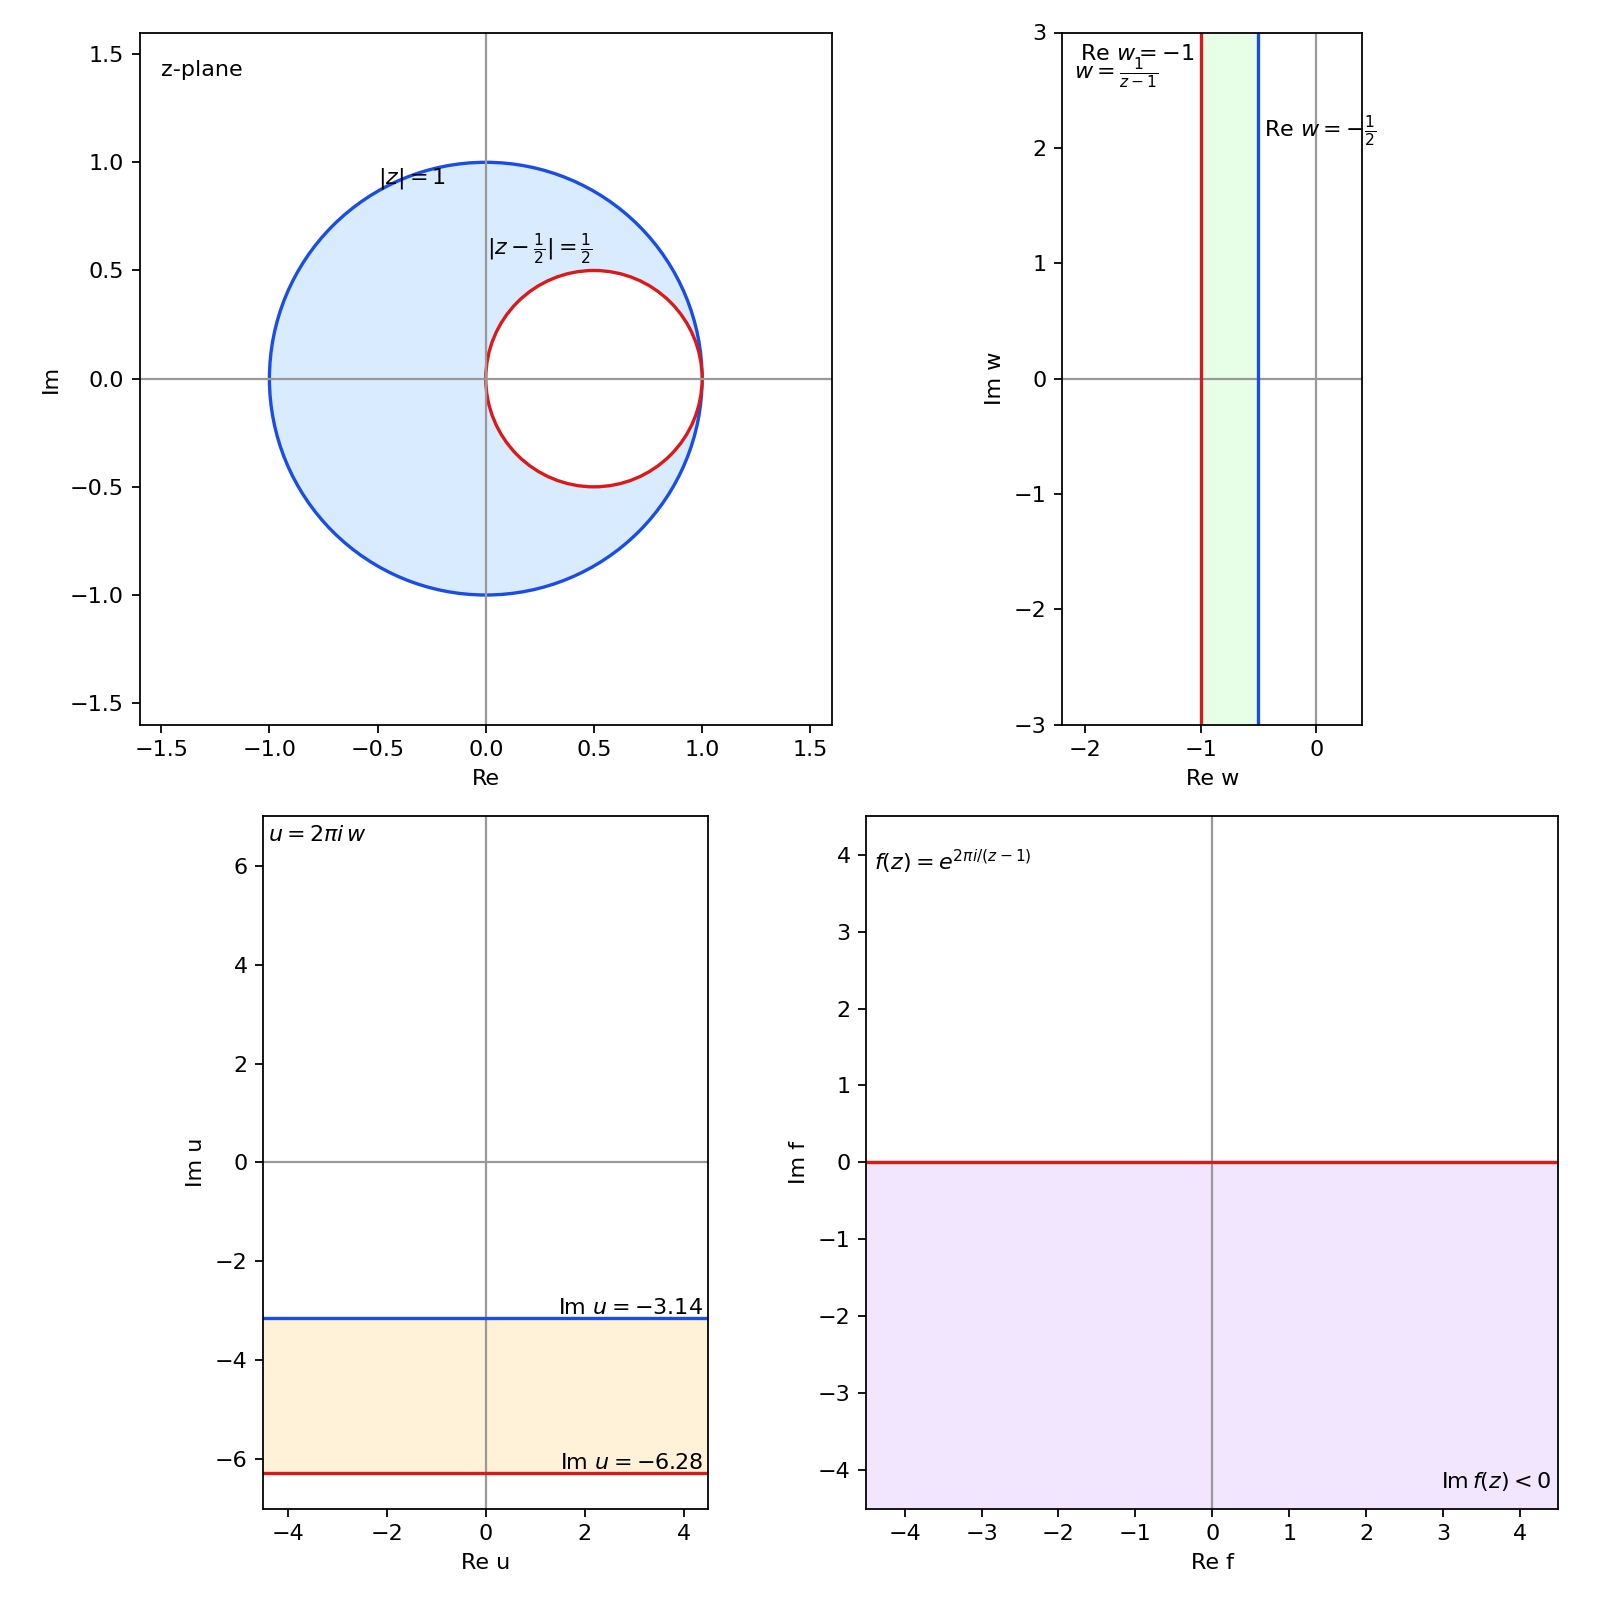
\includegraphics[scale=0.65]{conformal-mapping.png}
        \end{figure}
    \end{sol}
\end{exercise}

\section{Elementary Riemann Surfaces}
This is an optional section to introduce Riemann surfaces. We won't need this material, however.

The visualization of a function by means of the corresponding mapping is completely clear only when the mapping is one to one. If this is not the case, we can still give our imagination the necessary support by the introduction of generalized regions in which distinct points may have the same coordinates. In order to do this it is necessary to suppose that points which occupy the same place can be distinguished by other characteristics, for instance a tag or a color. Points with the same tag are considered to lie in the same \emph{sheet} or \emph{layer}.

This idea leads to the notion of a \emph{Riemann surface}, which is -- put simply -- a one-dimensional complex connected smooth manifold. For example, the Riemann sphere we have been dealing with all throughout this text is better known as $\CC\PP^1$, \emph{complex projective $1$-space}. With our construction, it is obvious that $\CC\PP^1$ is equivalent to a sphere, but this can be proven rigorously starting from its definition $$\CC\PP^1=\CC^2 \quotient \sim, \quad (z_1,z_2) \sim (z_1',z_2') \iff \dfrac{z_1}{z_1'}=\dfrac{z_2}{z_2'}.$$ Then $\CC\PP^1$ can be shown to be diffeomorphic to $S^2$. This requires familiarity with differential topology.

It is not our intention to give a rigorous definition of a Riemann surface; for our purposes it is sufficient to introduce it in a purely descriptive manner. The interested reader can follow up with a course on Riemannian geometry. For now, we content ourselves with some informally developed examples.

\begin{example}
    The simplest Riemann surface is connected with the mapping by a power $w=z^n$, where $n>1$ is an integer. We know that there is a one-to-one correspondence between each angle $(k-1)(2\pi/n)<\arg z<k(2\pi/n)$, $k=1,2,\dots,n$, and the whole $w$-plane except for the positive real axis. The image of each angle is thus obtained by performing a ``cut'' along the positive axis; this cut has an upper and lower ''edge.'' Corresponding to the $n$ angles in the $z$-plane we consider $n$ identical copies of the $w$-plane with the cut. They will be the ``sheets'' of the Riemann surface, and they are distinguished by a tag $k$ which serves to identify the corresponding angle. When $z$ moves in the plane, the point $w$ should be free to move on the Riemann surface. For this reason, we must attach the lower edge of the first sheet to the upper edge of the second, and so on. In the last step the lower edge of the $n$th sheet is attached to the upper edge of the first, completing the cycle. In a physical sense this is not possible without self-intersection, bu the idealized model shall be free from this discrepancy. The result of the construction is a Riemann surface whose points are in one-to-one correspondence with the points of the $z$-plane. What is more, this correspondence is continuous if continuity is defined in the sense suggested by the construction.

    The cut along the positive axis could be replaced by a cut along any simple arc from $0$ to $\infty$.

    The point $0$ is called a \emph{branch point} since it connects all the sheets. In general, if a point connects $h$ sheets, it is said to be a branch point of order $h-1$.
\end{example}

\begin{example}
    The Riemann surface corresponding to $w=e^z$ is of similar nature. In this case the function maps each parallel strip $(k-1)2\pi<y<k \cdot 2\pi$ onto a sheet with a cut along the positive axis. The sheets are attached to each other so that they form an endless screw. The origin will \textit{not} be a point of the Riemann surface, because $e^z$ is never zero.
\end{example}
